\documentclass[compress]{beamer}

\usetheme[light,lighttitle,framenumber]{UniversiteitAntwerpen}

\usepackage{lipsum}
\usepackage{outlines}
\usepackage{pgfpages}
\setbeameroption{show notes}

\newcommand{\slidetitle}[1]{\textbf{\Large{#1}}\vspace{5mm}}

\title{Chess AI: GrandQ}
\subtitle{5-Artificiële Intelligentie}

\author{Mathias Maes, Tijs Van Alphen\\ en Willem Van der Elst}

\begin{document}

\maketitle

\begin{frame}
    \slidetitle{GrandQ}
    \begin{outline}
        \1 Special Q-learner
            \2 Alpha-Beta pruning agent inside
        \1 Our project has 2 agents
        \1 Based on:
            \2 Mannen, H. (2003). \textit{Learning to play chess using reinforcement learning with database games}. Utrecht: Utrecht University. Retrieved 12 12, 2020, from \href{http://citeseerx.ist.psu.edu/viewdoc/download?doi=10.1.1.109.810&rep=rep1&type=pdf}{http://citeseerx.ist.psu.edu/viewdoc/download?doi=10.1.1.109.810\\\&rep=rep1\&type=pdf}
            \1 Git: \href{https://gitlab.com/Artificiele_Intelligentie/chess}{https://gitlab.com/Artificiele\_Intelligentie/chess}
    \end{outline}

\end{frame}

\begin{frame}
    \slidetitle{Alpha-Beta pruning agent}

    \begin{outline}
        \1 Normal alpha-beta pruning agent
        \1 Not a too complex evaluation function
    \end{outline}
\end{frame}

\begin{frame}
    \slidetitle{Q-Learning agent}
    \begin{outline}
        \1 Generalised Q-Learner
        \1 Highly optimized
            \2 Multi-threading
                \3 Mutex locking
            \2 Caching of states
        \1 Faster at calculating $\rightarrow$ Faster training
    \end{outline}
\end{frame}

\begin{frame}
    \slidetitle{Q-Learning agent: Features}
    \begin{outline}
        \1 Lots of features
            \2 Better understanding of environment
            \2 Alpha-Beta for predicting
        \1 Struggles with overlearning
            \2 Normalise input
            \2 $\sigma^*(x) = \frac{2}{1 + e^{-x}} -1: \sigma^*(x) \in \left]-1, 1\right[ $ 
            \3 Derived from $\sigma(x) = \frac{1}{1+e^{-x}}$
    \end{outline}
\end{frame}

\begin{frame}
    \slidetitle{Q-Learning agent: Training}

    \begin{outline}
        \1 Created convenient script
            \2 Changing variables quick (like max depth, epsilon, ...)
        \1 Trained on VPS
            \2 Google collab: slow with CPU driven programs
            \2 Microsoft Azure:
                \3 Ran on Free Credits
                \3 About a week
                \1 Opponents: Stockfish, Alpha-Beta, (GrandQ)
    \end{outline}

\end{frame}

\begin{frame}
    \slidetitle{Results and conclusion}

    \begin{minipage}{0.4\textwidth}
        \begin{flushleft}
            Stockfish
        \end{flushleft}
    \end{minipage}
    \hfill
    \begin{minipage}{0.4\textwidth}
        \begin{flushright}
            Alpha-Beta
        \end{flushright}
    \end{minipage}

    \begin{figure}[h]
        \begin{subfigure}
            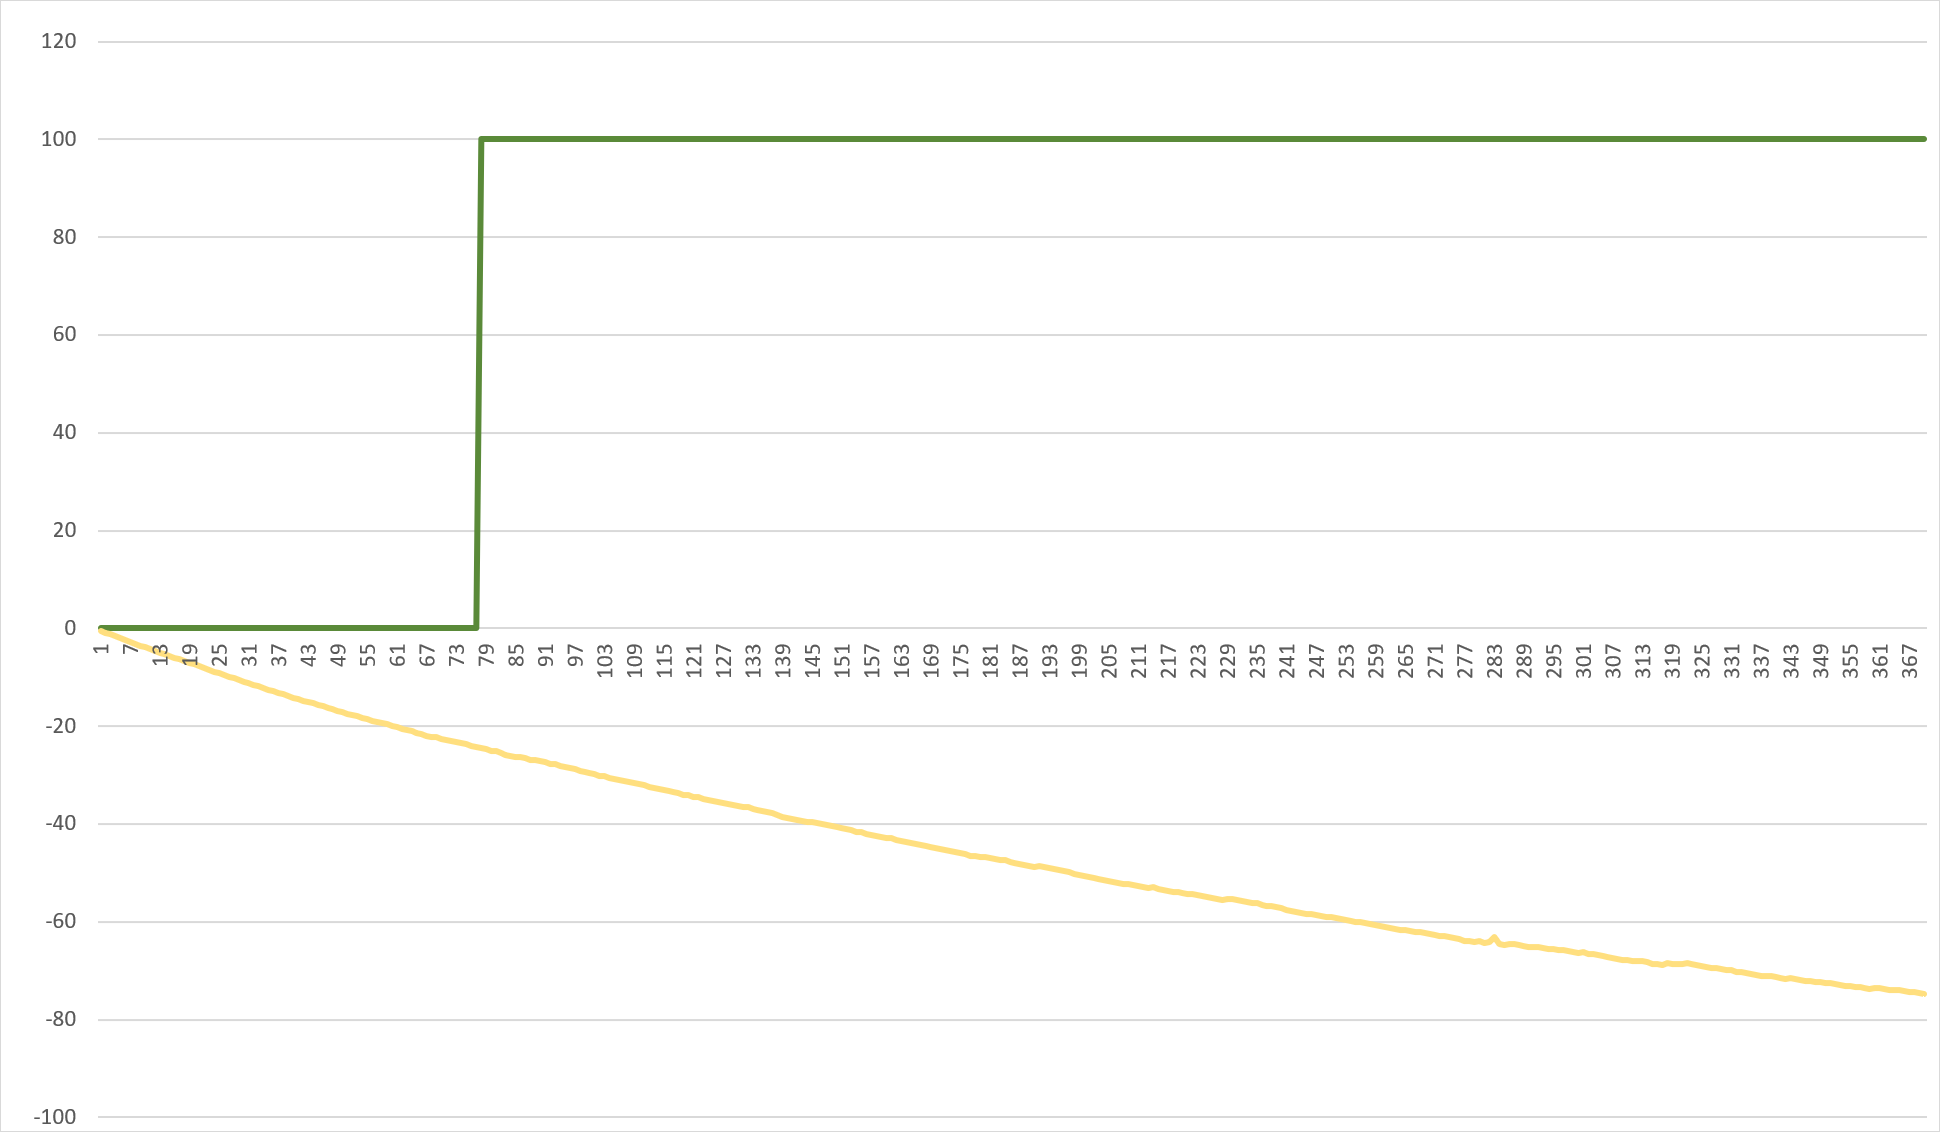
\includegraphics[height=75pt]{../Verslag/images/EXCEL_2020-12-12_18-01-10.png}
        \end{subfigure}
        \begin{subfigure}
            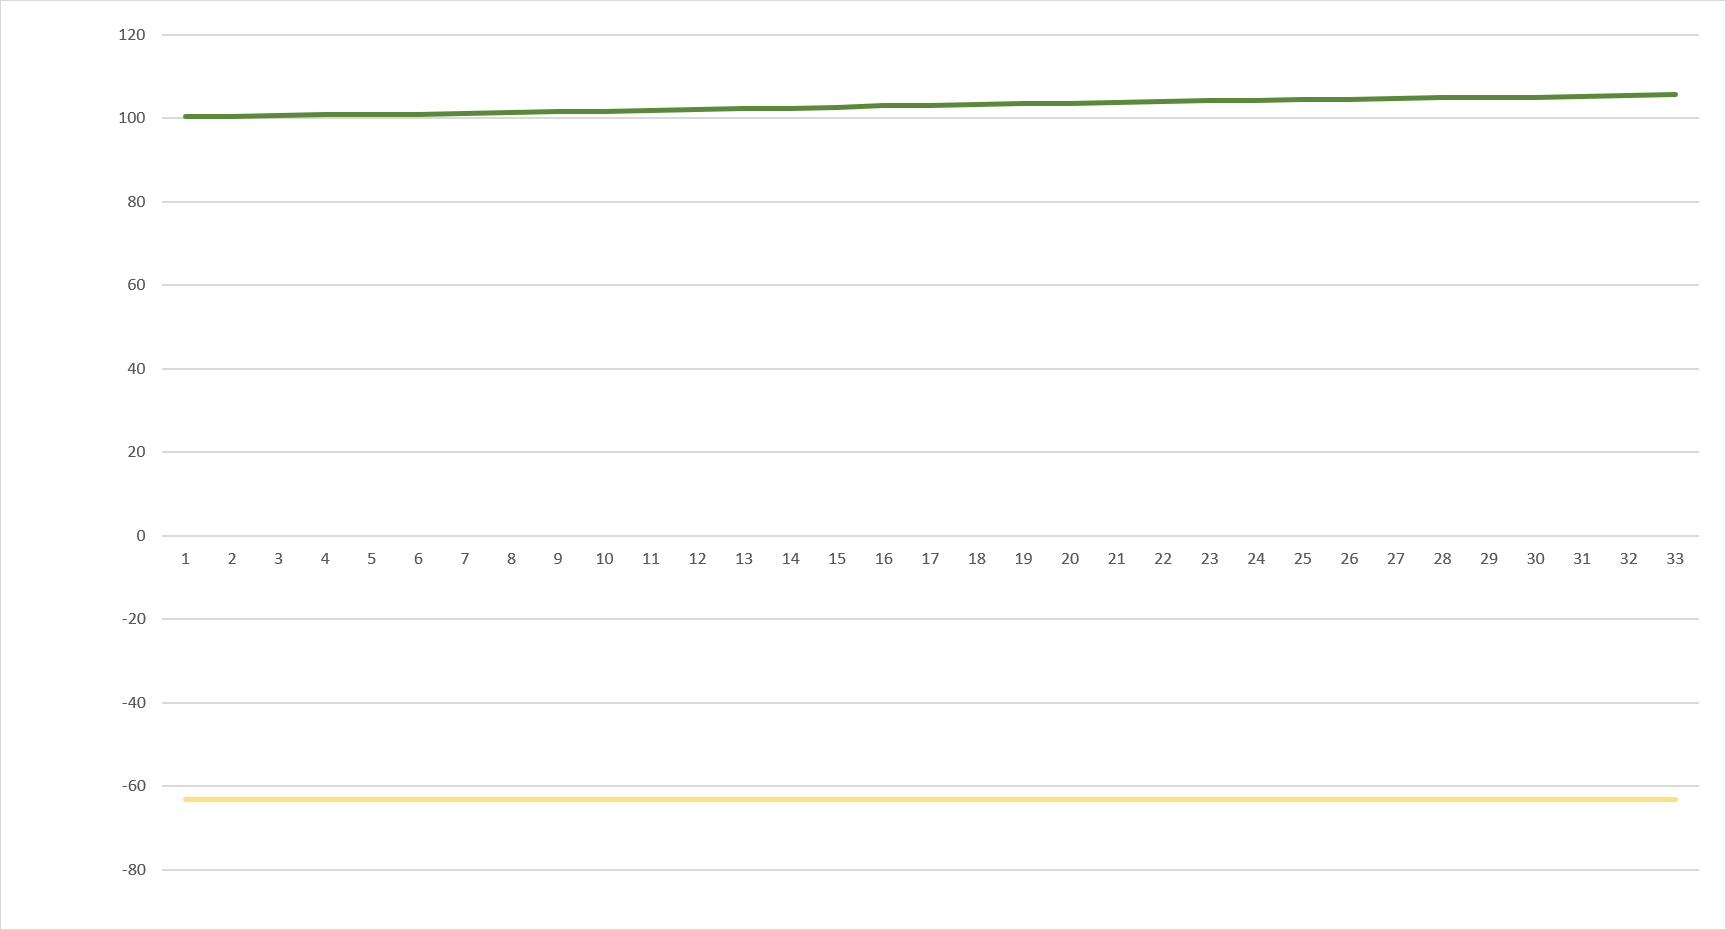
\includegraphics[height=75pt]{../Verslag/images/EXCEL_2020-12-12_17-58-38.png}
        \end{subfigure}
        \begin{subfigure}
            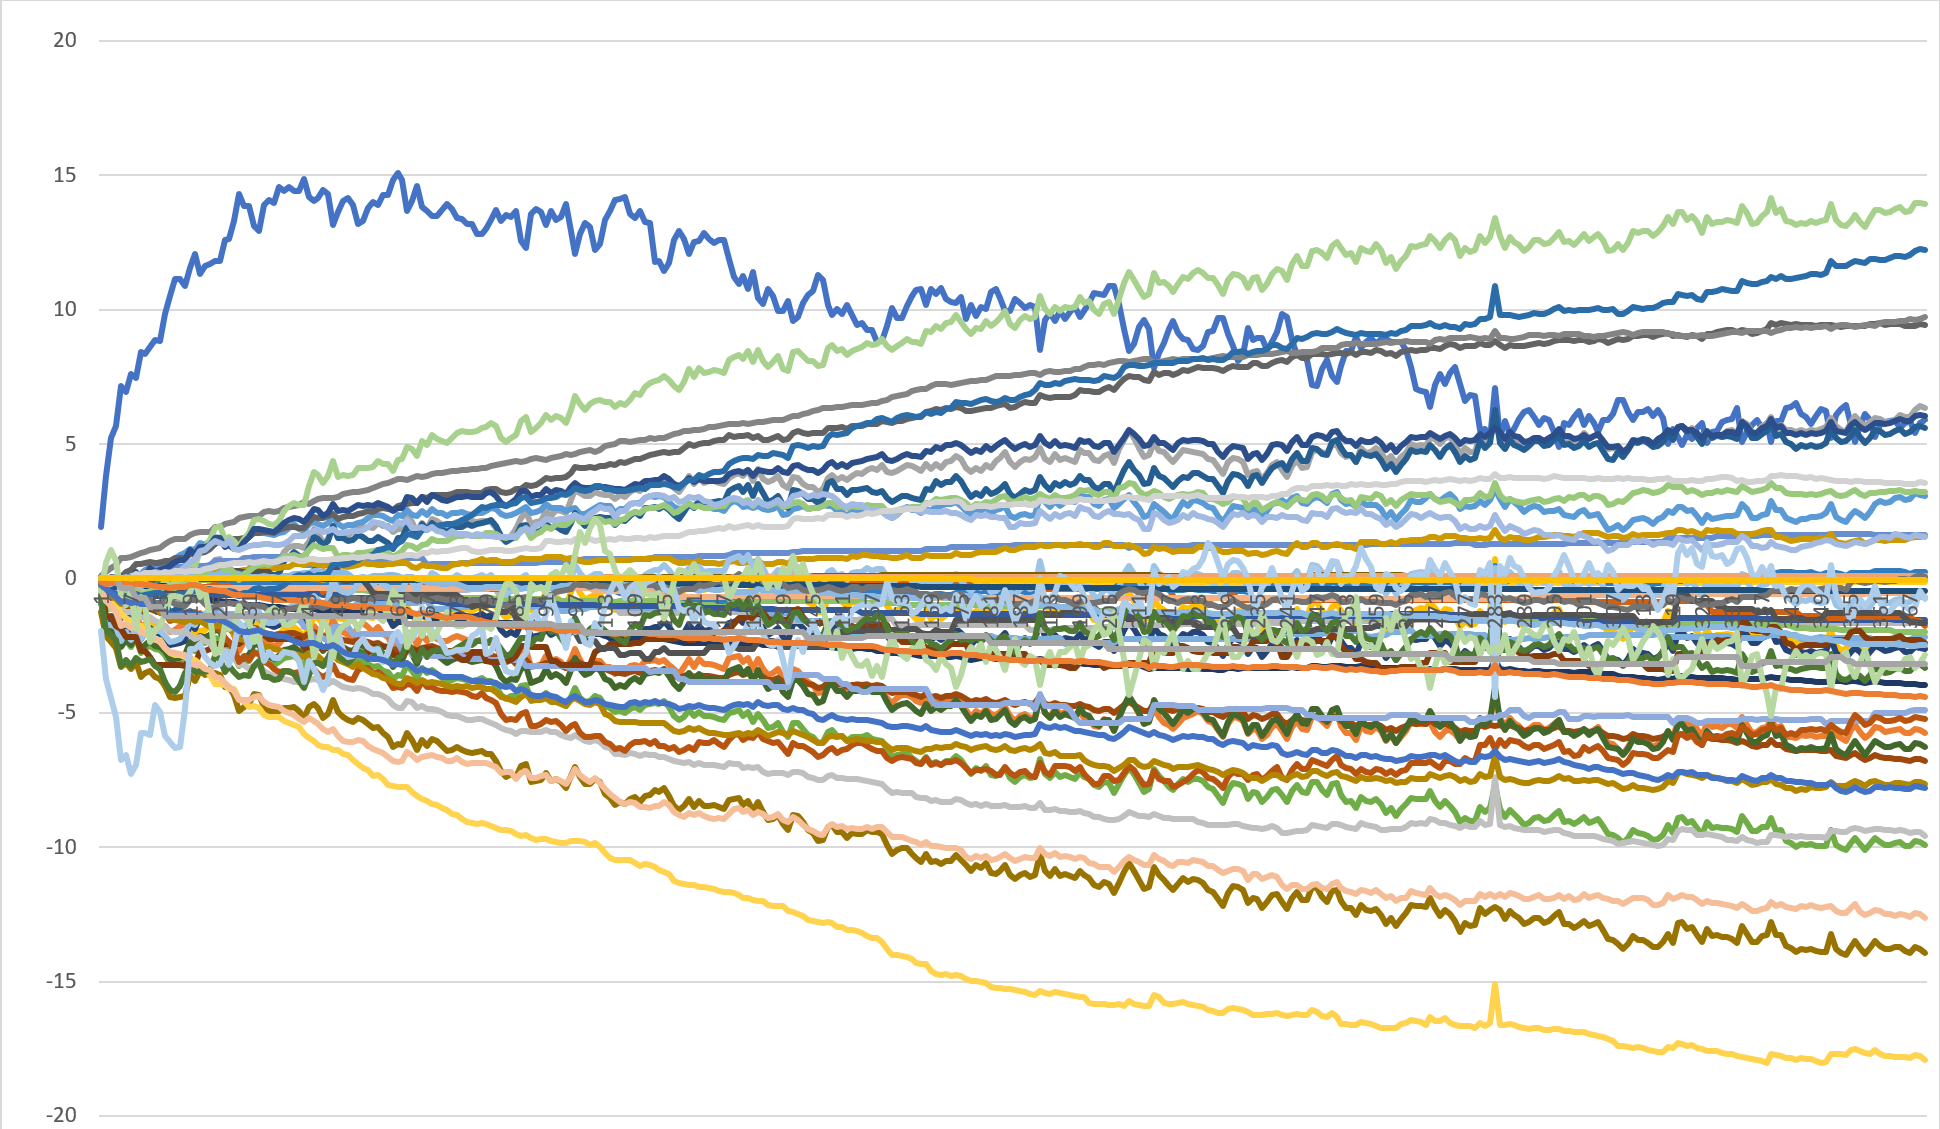
\includegraphics[height=75pt]{../Verslag/images/EXCEL_2020-12-12_18-01-58.png}
        \end{subfigure}
        \begin{subfigure}
            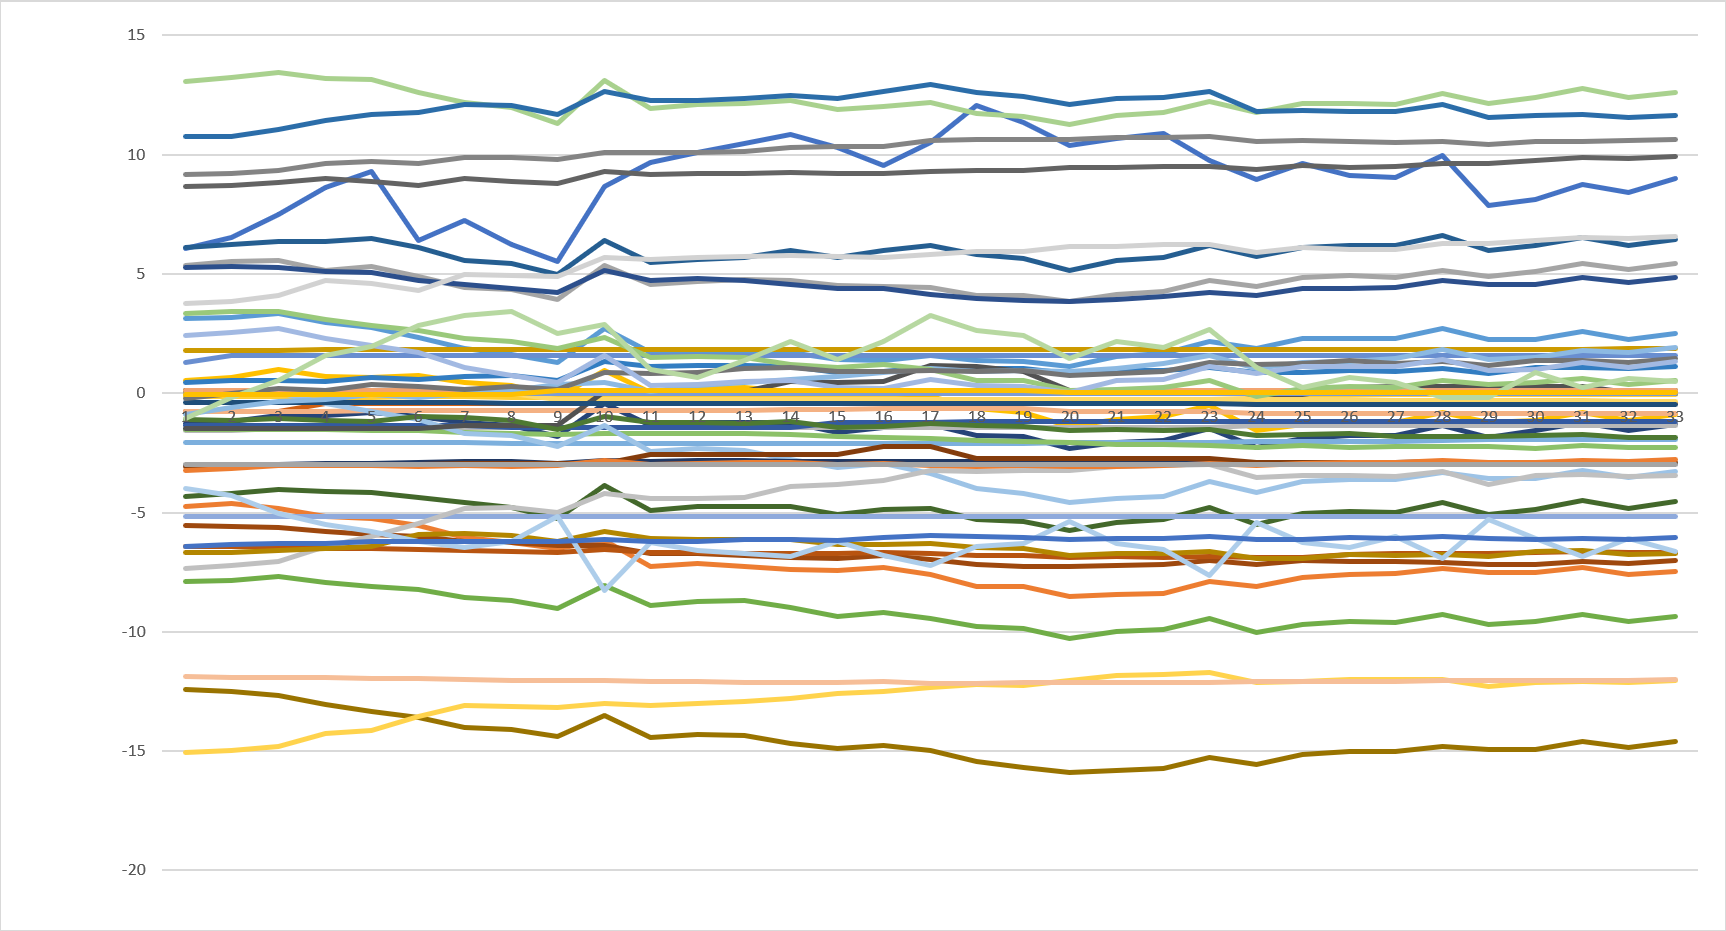
\includegraphics[height=75pt]{../Verslag/images/EXCEL_2020-12-12_18-02-40.png}
        \end{subfigure}
    \end{figure}
\end{frame}

\begin{frame}
    \slidetitle{Demo}
    \begin{outline}
        \1 GrandQ is open to play with on lichess
            \2 Possible to play against it yourself
        \1 \underline{\href{https://lichess.org/@/grandQ_AI}{https://lichess.org/@/grandQ\_AI}}
    \end{outline}
\end{frame}

\end{document}
